\documentclass[11pt]{article}
\usepackage{amsmath}
\usepackage{amssymb}
\usepackage{amscd}
\usepackage{graphicx}
\graphicspath{ {./images/} }

\title{Neural network knowledge distillation in tensor networks}
\author{Dereck Piché}
\date{\today}
\begin{document}
\maketitle
\begin{abstract}
\end{abstract}

\section{Introduction}
In the last few decades, the use of artificial neural networks has gained a lot of popularity in several application areas. Because of their usefulness, we would like to be able to use them in systems that have fewer computational resources (nested systems, for example). Thus, we would like to find methods to reduce their temporal and spatial complexity while keeping their capabilities. This is where knowledge distillation comes in. Suppose we have a trained neural network that performs well on a certain task T. Then we can say that this neural network has knowledge about this task T. We would like to be able to transfer the knowledge of an already trained neural network into a system that takes less space. The technical term given to the knowledge transfer process is knowledge distillation. Despite the youth of this avenue of study, it remains broad in scope. The project will therefore focus more specifically on knowledge distillation of artificial neural networks in tensor networks. 
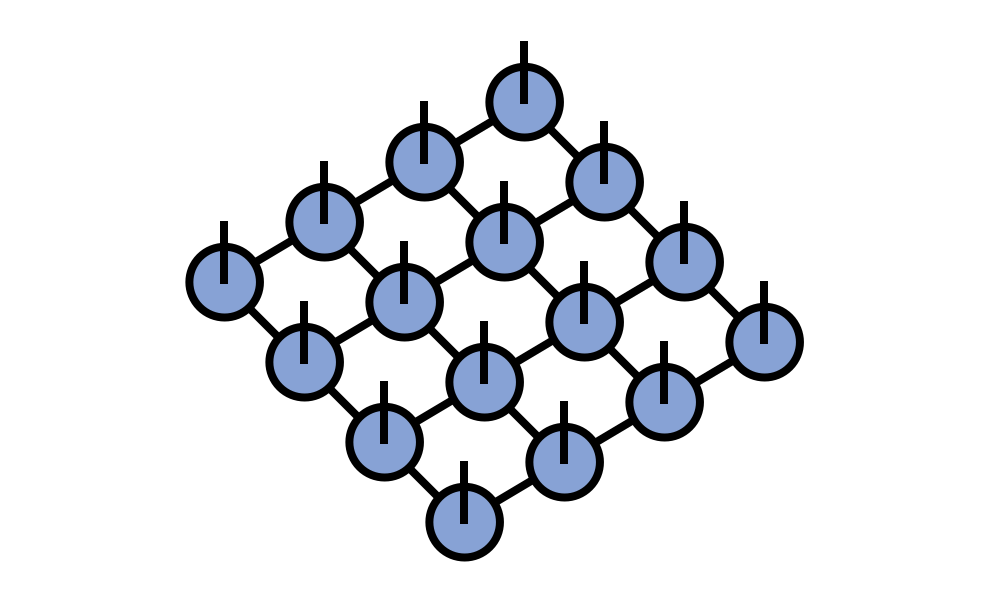
\includegraphics{PEPS}
We now need to briefly explain what a tensor network is. Tensor networks are mathematical objects originating from the modeling of quantum phenomena (see Richard Penrose and Feynman). Here we see tensors as a generalization of vectors and matrices where we have an arbitrary number of indices. It is important to mention that tensor networks are intimately linked to a graphical notation which allows us to manipulate them much more easily than if we were limited to a purely analytical notation. From this notation, researchers have created different types (or patterns or categories) of tensor networks that possess certain distinct properties. Some of these patterns (such as the MPS https://tensornetwork.org/mps/) possess properties that are crucial to our task. In particular, several factorization and optimization methods for temporal and spatial complexity are known and studied for MPS (Matrix Product State / Tensor Train). Thus, we could use these optimizations after distillation to reduce the computational costs of neural networks. The project will consist of analyses and experiments that will aim to clarify/advance this topic (in the form of a report). We have not determined how theoretical or practical the project will be.

\section{Learning Tensors Networks and Deep Neural Networks}
First, we must clearly distinguish the two approaches before trying to convert one to the other. The main difference between Deep Neural Networks is in the order of the transformation. In the forward pass of a Learning Tensor Network, the transformation must be applied directly to the inputs before being actualised as elements of the tensor network. The learning procedure can then be applied. It is done "apriori". In Neural Networks, this is done at multiple steps in the network. 

\section{Convolutional Neural Networks}
We could reproduce the filters of CNN's by applying a Kronecker product of the feature map $[ 1, \ \ x ]^T $ on a group of locally bound functions. In turn, we use this to create a new map.

\section{Direct weight optimization approach}
We propose to distill knowledge into a student by directly taking a NN parent model and refactoring it's linear properties by use of tensor network methods. The method is less akin to teaching, and more with factorisation. In the paper https://arxiv.org/pdf/2207.02851.pdf (page 3), it is proposed that each vector of the weight matrices would be decomposed into a MPS. We would rather decompose the weight matrice directly. It was also proposed that the each vector space mapping of the layers of the neural network would be factorised used MPS. This is an interesting idea that while simple deserves some experimental exploration.

\section{Locality}
Convolutional Neural Networks bringed a new idea to the table, the idea of locality. Structured data comes with position-based information. 
As such, we shall try to improve the by using tensor product. 

\section{Layer-by-layer approach}
It has been common to each layer of a neural network as a certain abstracted representation of the previous information and their for generalisibility. Thus, we propose to change the cost, we use a tensor for multilinear mapping and train each mapping individualy according to the output of it's paired set of layers. 
\begin{equation*}
\begin{CD}
    x @>>>H_1 @>>>H_2 @>>>(\dots)@>g>> \hat{y}
\end{CD}
\end{equation*}
Each hidden layer is of the form;
\begin{equation*}
    a^l = \sigma^l \bigl( W^l a^{l-1} \bigr)
\end{equation*}
In tensor layer form, it will be defined as 
\begin{equation*}
    a^l = T^l \cdot \Phi \bigl( a^{l-1} \bigr)
\end{equation*}b
The main difference is that in the tensor approach, the "heavy" part is done by the non-linear transformation while a little work is done with the linear mapping. The opposite is true with neural networks. Here, $\Phi(X)$ (X begin the input vector) is a tensor product of several identical non-linear mappings of each element $x_i$. Thus, we have 
\begin{equation*}
    \Phi(X) = \phi(x_1)\phi(x_2)\dots\phi(x_n)
\end{equation*}
Were each $\phi : \mathbb{R} \rightarrow \mathbb{R}^d$, and each $d > 1$. Thus, our $\Phi(X) : \mathbb{R}^n \rightarrow \mathbb{R}^{ (d \times)^{n-1}d} $. In other words, our $\Phi$ returns a tensor of order $n$, where each indices run from $1$ to $d$.




\bibliography{simple}

\end{document}
This is never printed
